\part{State of the Art}

\chapter{Digital Twins in Industry}

This part reviews concrete previous works that are close to the technological foundations of a smart irrigation digital twin system. It begins with industrial digital twins, because Industry 4.0 provides many mature examples of synchronization between a physical asset and a virtual model. It then moves to smart agriculture and irrigation systems, before focusing on digital twins applied to agriculture and water management. The selected works are implementation, prototype, simulation, or case-study papers. Review and survey papers are not used as main state-of-the-art papers in this part.

\section{Cyber-Physical Production Systems}

\subsection[The Digital Twin: Realizing the Cyber-Physical Production System for Industry 4.0]{The Digital Twin: Realizing the Cyber-Physical Production System for Industry 4.0 \cite{uhlemann2017digitalTwinCPPS}}

\subsubsection{Overview}

Uhlemann et al. address the problem of connecting a physical production system with a digital representation in the context of Industry 4.0. The paper is relevant because it treats the digital twin as a practical mechanism for realizing a cyber-physical production system, rather than as a purely conceptual model. The physical asset is an industrial production environment, while the digital counterpart is used to represent and analyze production behavior.

\subsubsection{Architecture / Methodology}

The methodology is organized around the link between a physical production system and its virtual counterpart. The physical side contains the machines, production resources, and shop-floor events. The digital side receives data from these resources and uses them to keep an updated representation of the production state.

The important point in this paper is the data flow. Measurements and events are not treated as isolated monitoring values. They are used to update the virtual model so that the model reflects what is happening in the production system. This is the difference between a simple dashboard and a digital twin: the virtual representation must be continuously informed by the physical process.

The paper also shows that the digital twin has a decision-oriented role. Once the virtual model is synchronized with the physical system, it can be used to understand production behavior, detect deviations, and support operational decisions. For this thesis, the same logic can be translated to irrigation: field sensors feed a virtual state, and the virtual state supports water-management decisions.

\subsubsection{Evaluation and Results}

The paper presents a concrete cyber-physical production-system realization and uses it to illustrate how digital twin data can support monitoring and production understanding. The available verified metadata does not expose detailed numerical performance metrics such as latency, prediction accuracy, or throughput improvement. Therefore, in this review the validation is treated as qualitative prototype validation.

\subsubsection{Limitations and Relevance to This Project}

The main limitation is that the paper is focused on industrial production and does not address uncertain biological processes such as soil moisture dynamics, crop water demand, or weather variability. However, it is useful because it clarifies the core digital twin pattern: a physical asset must continuously inform a virtual representation, and the virtual representation must support decisions. The remaining gap for irrigation is to adapt this pattern to field sensing, water management, and agronomic decision support.

\section{Visualization and Human Interaction}

\subsection[Visualising the Digital Twin Using Web Services and Augmented Reality]{Visualising the Digital Twin Using Web Services and Augmented Reality \cite{schroeder2016visualisingDigitalTwin}}

\subsubsection{Overview}

Schroeder et al. study how a digital twin can be visualized and accessed by users through web services and augmented reality. The paper is important because digital twins are not only data models; they also need interfaces that allow operators to understand the state of the physical system. In industrial monitoring, this interaction layer helps users interpret data and inspect the virtual representation of equipment.

\subsubsection{Architecture / Methodology}

The methodology separates the digital twin system into several clear layers. The first layer is the physical industrial asset, which produces operational data. The second layer is the digital representation, where the state of the asset is modeled and made available to external services. The third layer is the web-service interface, which exposes the digital twin data in a structured way.

The final layer is the augmented-reality visualization. Instead of showing only numerical values, the system allows the user to inspect information through a visual interface connected to the asset. This makes the digital twin easier to understand for an operator, especially when the physical object and its digital information must be interpreted together.

This paper is useful because it treats visualization as part of the digital twin methodology. A virtual model is not sufficient if users cannot interpret it. In a smart irrigation system, the same principle applies: soil moisture values, irrigation state, and recommendations must be displayed in a way that helps the user understand the field situation.

\subsubsection{Evaluation and Results}

The work is evaluated as a prototype that demonstrates the feasibility of visualizing a digital twin through web services and augmented reality. The paper validates the interaction concept qualitatively. The available verified metadata does not provide exact numerical values for response time, usability scores, or industrial productivity gains.

\subsubsection{Limitations and Relevance to This Project}

The limitation is that the contribution is mainly centered on visualization and interaction, not on predictive modeling or automatic control. For a smart irrigation digital twin, this work remains relevant because farmers and operators also need clear interfaces to understand sensor data, virtual states, and recommendations. The gap is the integration of visualization with irrigation-specific prediction, scheduling, and control.

\section{Production Management and Control}

\subsection[Digital Twin-Based Smart Production Management and Control Framework for the Complex Product Assembly Shop-Floor]{Digital Twin-Based Smart Production Management and Control Framework for the Complex Product Assembly Shop-Floor \cite{zhuang2018digitalTwinAssembly}}

\subsubsection{Overview}

Zhuang et al. propose a digital twin framework for smart production management and control in a complex product assembly shop floor. The work is relevant because it goes beyond simple visualization and uses the digital twin as a management and control support layer. The physical asset is an assembly shop floor, and the virtual model represents the state of the assembly process.

\subsubsection{Architecture / Methodology}

The paper identifies four main methodological blocks. The first block is the real-time acquisition, organization, and management of physical shop-floor data. This block is responsible for collecting data from the assembly environment and preparing it so that it can be used by the digital twin.

The second block is the construction of the assembly shop-floor digital twin. This virtual representation models the resources, state, and behavior of the assembly process. It is not only a static model of the factory layout; it is designed to reflect the current production situation.

The third block is prediction based on the digital twin and big-data methods. The digital twin provides structured production-state information, while the prediction layer uses this information to anticipate production behavior. The fourth block is the management and control service layer, which transforms analysis results into operational support for the shop floor.

The implementation scenario is a satellite assembly shop floor. This example shows how a digital twin can support a complex process where many resources, operations, and constraints must be coordinated. For irrigation, the equivalent methodological chain is sensor acquisition, field-state modeling, water-need prediction, and irrigation decision support.

\subsubsection{Evaluation and Results}

The paper validates the framework through an assembly shop-floor scenario. The evaluation demonstrates that digital twin modeling can support production management and control by connecting real production data with predictive and service functions. The verified public information does not provide detailed numerical performance values, so this review treats the reported validation as scenario-based and qualitative.

\subsubsection{Limitations and Relevance to This Project}

The limitation is that the framework is designed for manufacturing operations where the production process is more controlled than an agricultural field. It does not address weather uncertainty, soil heterogeneity, or plant response. Its relevance is strong at the architectural level: a smart irrigation digital twin also needs data acquisition, virtual modeling, prediction, and decision services. The remaining gap is to translate this layered industrial logic into a practical irrigation workflow.

\section{Open-Source Smart Manufacturing}

\subsection[An Open Source Approach to the Design and Implementation of Digital Twins for Smart Manufacturing]{An Open Source Approach to the Design and Implementation of Digital Twins for Smart Manufacturing \cite{damjanovic2019openSourceDigitalTwins}}

\subsubsection{Overview}

Damjanovic-Behrendt and Behrendt propose an open-source approach for designing and implementing digital twins in smart manufacturing. This paper is relevant because it focuses on implementation choices, not only on abstract digital twin definitions. In industrial systems, open-source components can reduce vendor lock-in and make the digital twin architecture easier to reproduce.

\subsubsection{Architecture / Methodology}

The methodology is implementation-oriented. The authors focus on how a digital twin can be built with open-source components rather than only describing a conceptual architecture. This makes the paper useful for projects that need a practical and reproducible system design.

The physical manufacturing resources provide the operational data. These data are connected to digital representations through software services. The digital twin layer then organizes the information so that it can be accessed by applications that support monitoring, analysis, and decision-making.

The paper also emphasizes interoperability. In smart manufacturing, different machines, protocols, and software services must communicate. The open-source approach is therefore not only a cost decision; it is a way to make the system easier to integrate, extend, and reproduce.

For a smart irrigation digital twin, this methodology suggests that the architecture should be modular. Sensors, backend services, database components, prediction modules, and user interfaces should communicate through clear interfaces so that the system can evolve without being rebuilt from zero.

\begin{figure}[H]
    \centering
    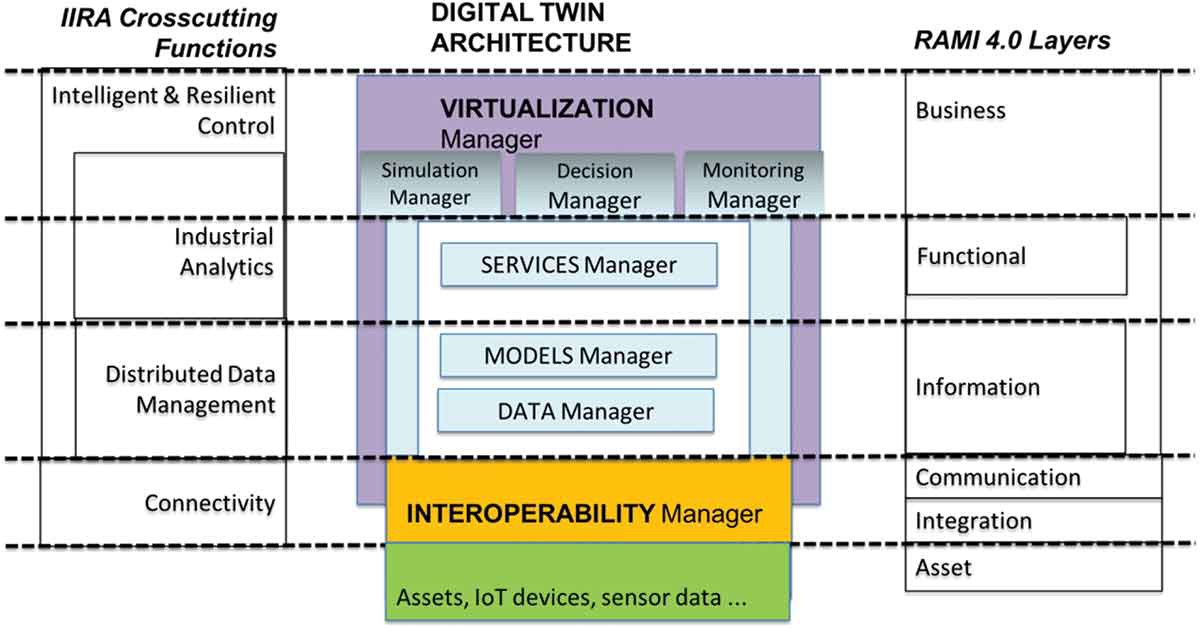
\includegraphics[width=0.75\textwidth]{figures/chapter_03/chapter 3.4.jpg}
    \caption{Open-source digital twin implementation approach for smart manufacturing, adapted from \cite{damjanovic2019openSourceDigitalTwins}. Source: \url{https://doi.org/10.1080/0951192X.2019.1599436}.}
    \label{fig:soa_damjanovic_open_source_dt}
\end{figure}

\subsubsection{Evaluation and Results}

The paper provides an implementation case for smart manufacturing. The validation is mainly architectural and prototype-oriented. The available verified metadata does not expose exact numerical metrics such as prediction accuracy, downtime reduction, or throughput improvement, so the result is considered qualitative validation of an open-source implementation path.

\subsubsection{Limitations and Relevance to This Project}

The limitation is that the work targets manufacturing systems, not agriculture. It also does not focus on irrigation decisions, agronomic constraints, or water-saving metrics. Its relevance lies in the engineering approach: open-source components, modular services, and reproducible implementation are useful for building practical digital twin systems outside industry. The gap remains the adaptation of these implementation ideas to IoT sensing, irrigation scheduling, and water management.

\section{Discussion}

The four industrial papers show a progression from synchronization between a physical production system and a virtual representation, to visualization, prediction, management, and implementation. They are useful because they demonstrate that a digital twin is not a single algorithm. It is a system that connects data acquisition, virtual modeling, decision support, and sometimes control. However, these works are situated in industrial environments where assets and processes are more stable than agricultural systems. Agriculture adds uncertainty from weather, soil, crop growth, and water availability.

\begingroup
\scriptsize
\setlength{\tabcolsep}{1pt}
\begin{longtable}{@{}>{\raggedright\arraybackslash}p{0.12\textwidth}>{\raggedright\arraybackslash}p{0.11\textwidth}>{\raggedright\arraybackslash}p{0.13\textwidth}>{\raggedright\arraybackslash}p{0.11\textwidth}>{\raggedright\arraybackslash}p{0.13\textwidth}>{\raggedright\arraybackslash}p{0.11\textwidth}>{\raggedright\arraybackslash}p{0.13\textwidth}>{\raggedright\arraybackslash}p{0.13\textwidth}@{}}
\caption{Comparison of selected industrial digital twin papers}\\
\toprule
Paper & Industrial domain & Digital twin purpose & Data source & Modeling / AI method & Validation & Main result & Limitation \\
\midrule
\endfirsthead
\toprule
Paper & Industrial domain & Digital twin purpose & Data source & Modeling / AI method & Validation & Main result & Limitation \\
\midrule
\endhead
Uhlemann et al. \cite{uhlemann2017digitalTwinCPPS} & Cyber-physical production & Realize Industry 4.0 production-system twin & Shop-floor production data & Virtual production-system representation & Prototype demonstration & Shows how CPPS data can feed a digital counterpart & No agricultural or water-management context \\
Schroeder et al. \cite{schroeder2016visualisingDigitalTwin} & Industrial monitoring & Visualize digital twin state & Web-service data from physical asset & Service-based representation and AR visualization & Prototype demonstration & Provides an interaction layer for digital twin inspection & Limited focus on prediction and control \\
Zhuang et al. \cite{zhuang2018digitalTwinAssembly} & Complex assembly shop floor & Production management and control & Real-time shop-floor data & Digital twin plus big-data-driven prediction & Assembly scenario & Connects data acquisition, twin model, prediction, and control services & Manufacturing assumptions do not transfer directly to fields \\
Damjanovic-Behrendt and Behrendt \cite{damjanovic2019openSourceDigitalTwins} & Smart manufacturing & Open-source digital twin implementation & Industrial system data & Modular open-source implementation & Implementation case & Supports reproducible smart-manufacturing twin design & Does not target irrigation or agronomic decisions \\
\bottomrule
\end{longtable}
\endgroup

The main gap identified from the industrial literature is the need to adapt mature digital twin principles to agricultural constraints. Industrial digital twins show strong patterns for synchronization, service layers, and decision support, but they do not solve the specific problems of irrigation: sparse field sensing, environmental variability, water balance, and user-oriented irrigation control.
